\documentclass{article}
\usepackage[T1]{fontenc}
\usepackage{lmodern}
\usepackage{pdfpages}


\newcommand{\subsectiontitlepage}[1]{%
  \clearpage
  \refstepcounter{subsection}%
  \phantomsection
  \addcontentsline{toc}{subsection}
    {\texorpdfstring{\protect\numberline{\thesubsection}#1}{#1}}
  \vspace*{\fill}
  \begin{center}
    {\huge\bfseries \thesubsection\quad #1\par}
  \end{center}
  \vspace*{\fill}
  \clearpage
}

\newcounter{savepage}
\newcommand{\includepdfnopagenum}[2][]{%
  \begingroup
    \setcounter{savepage}{\value{page}}%
    \includepdf[pagecommand={\thispagestyle{empty}},#1]{#2}%
    \setcounter{page}{\value{savepage}}%
  \endgroup
}

\usepackage{float}
\usepackage[ngerman]{babel}

\addto\captionsngerman{%
  \renewcommand{\figurename}{Abb.}%
}

\addto\captionsngerman{%
  \renewcommand{\tablename}{Tab.}% 
}

\usepackage{microtype}

\usepackage[letterpaper, top=1.0in, bottom=1.0in, left=1.0in, right=1.0in, heightrounded]{geometry}

\usepackage{enumitem}
\setlist[itemize]{left=1.5em,topsep=2pt,itemsep=3pt,parsep=0pt}
\setlist[enumerate]{left=1.5em,topsep=2pt,itemsep=2pt}

\usepackage{svg}

\usepackage{tabularx}
\usepackage{booktabs}
\usepackage[table,xcdraw]{xcolor}
\renewcommand{\arraystretch}{1.2}

\usepackage{tikz}
\usetikzlibrary{shapes, arrows, positioning, calc}

\tikzset{
  block/.style = {draw, rounded corners, align=center, minimum width=2.5cm, minimum height=1cm},
  arrow/.style = {->, thick}
}

\usepackage{titling}
\pretitle{%
  \vspace*{0.2\textheight}
  \centering
  
\includegraphics[width=0.8\textwidth]{SensorBear_Logo.png}\\[4mm]
  \LARGE
}
\posttitle{\par\vspace{8mm}}
\preauthor{\centering\Large}
\postauthor{\par\vspace{8mm}}
\predate{\centering\Large}
\postdate{\par}


\usepackage[hidelinks]{hyperref}
\usepackage{bookmark}
\hypersetup{
  pdftitle={Project Management Report},
  pdfauthor={Matthias Gregorich, Daniel Nebel, Viktor Novak, Damjan Petrovic, Marc Schneeweis},
  pdfcreator={LaTeX},
  pdfborder={0 0 0}
}

\newcommand{\branch}[1]{\texttt{#1}}

\title{Project Management Report}
\author{Matthias~Gregorich\\Daniel~Nebel\\Viktor~Novak\\Damjan~Petrovic\\Marc~Schneeweis}
\date{21.10.2025}

\begin{document}
\maketitle
\thispagestyle{empty}

\clearpage

\setcounter{tocdepth}{2}
\setcounter{secnumdepth}{2}

\pagenumbering{roman}
\tableofcontents
\clearpage

\pagenumbering{arabic}
\setcounter{page}{1}




\section{Product}
\subsection{Definition of Done}
Dieses Projekt ist fertig so bald Bearingpoint die vollständig funktionsfähigen ESP32 Geräte hat, die alle spezifizierten Funktionen gemäß den technischen Anforderungen erfüllen, erfolgreich durch das Backend mit den verschiedenen Frontends (Web, Mobile, Desktop) kommunizieren und alle Meilensteile bereits erreicht und dokumentiert worden sind und das Projekt spätestens am 8. April 2026 abgeschlossen ist.

\subsection{Deadlines}
\begin{figure}[H]
  \centering
  \includesvg[width=\textwidth]{DeadlinesTimelineCycle}
  \caption{Deadlines-Übersicht}
  \label{fig:deadlines}
\end{figure}



\subsection{Partner}

\begin{figure}[h]
  \centering
  \includesvg[width=0.45\textwidth]{BearingPoint_logo} 
  \caption{Logo von BearingPoint}
  \label{fig:bearingpoint-logo}
\end{figure}


\noindent
Der Partner und Auftraggeber dieses Projekts ist \textbf{BearingPoint}, eine international tätige Management- und Technologieberatung mit europäischen Wurzeln. 
Sie unterstützen Unternehmen bei der Umsetzung digitaler Lösungen mit den Schwerpunkten Software Engineering und Data Analytics.
BearingPoint verbindet Beratung mit eigenen IP-basierten Lösungen und arbeitet mit Technologiepartnern wie SAP, Microsoft und Salesforce zusammen. 
Betreute Branchen sind u.\,a.\ Finanzdienstleistungen, Telekommunikation, Energie/Versorger und Transport/Logistik.



\subsection{UI-Mockups}

\begin{figure}[H]
  \centering
  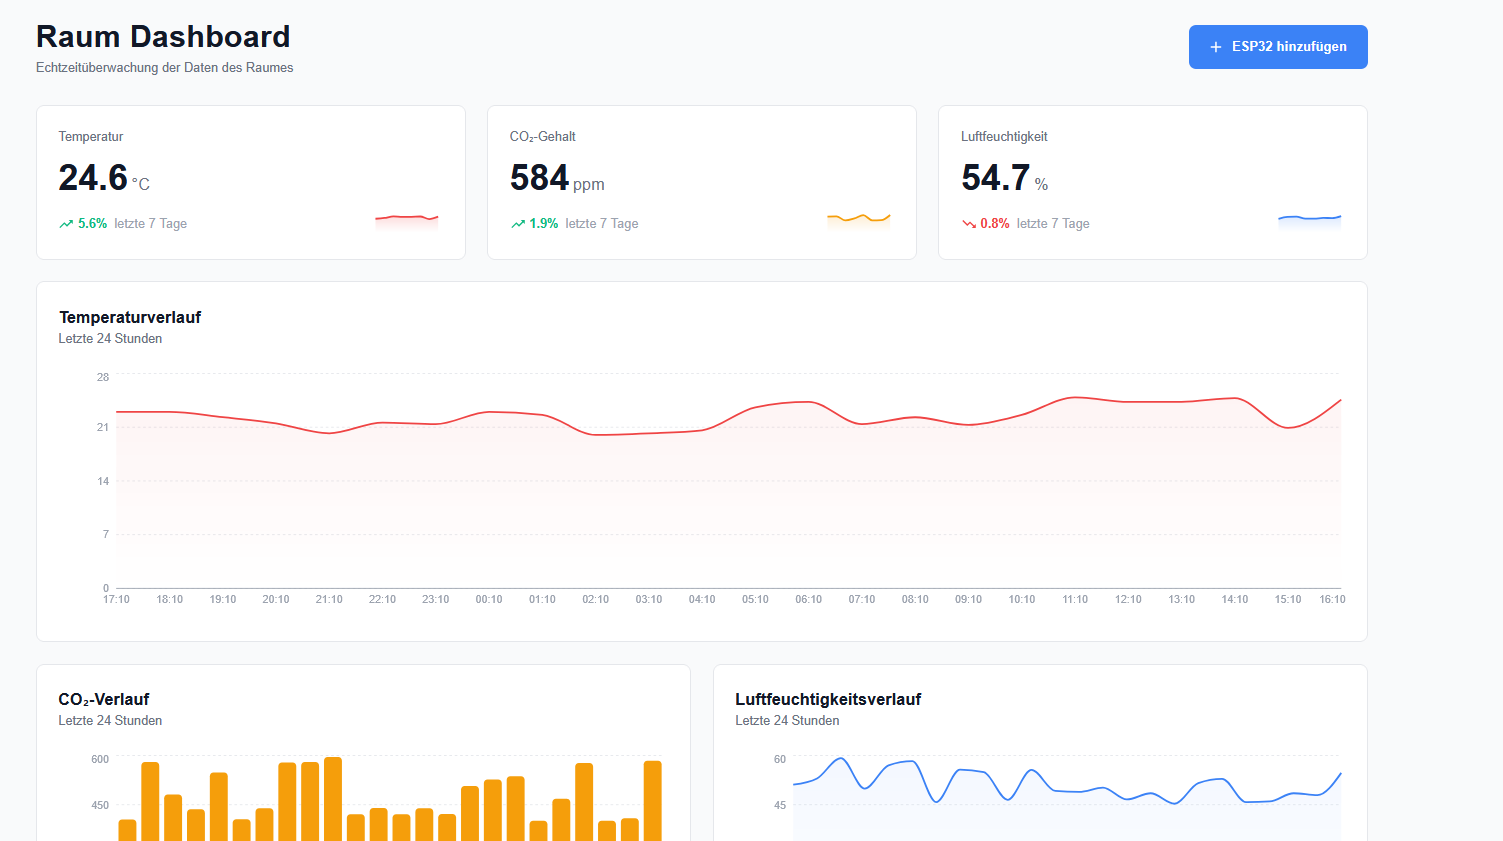
\includegraphics[width=\textwidth]{UI_Mockup_Web.png}
  \caption{UI-Mockup für die Web-Version (Landingpage)}
  \label{fig:ui-mockup-web}
\end{figure}

\begin{figure}[H]
  \centering
  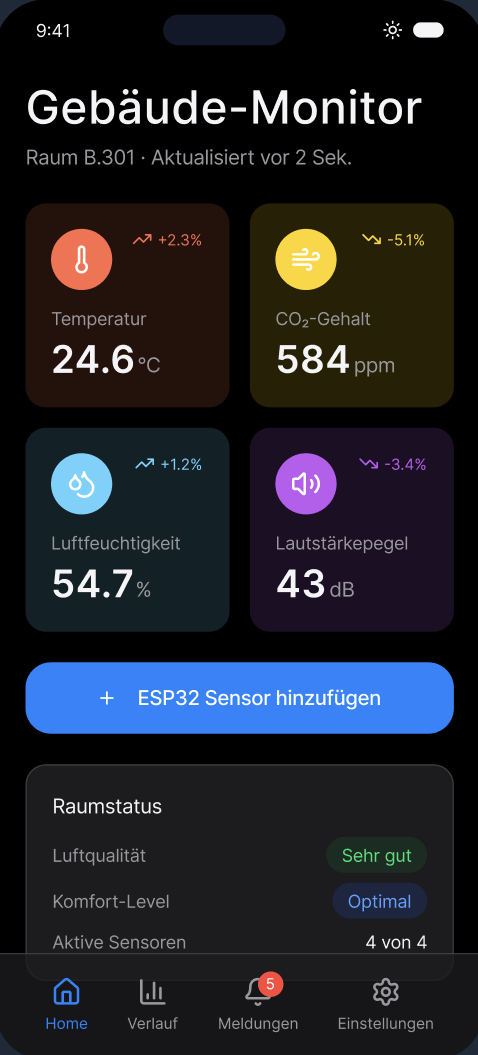
\includegraphics[width=\textwidth, height=0.9\textheight, keepaspectratio]{UI_Mockup_IOS.png}
  \caption{UI-Mockup für die IOS-Version (Landingpage)}
  \label{fig:ui-mockup-ios}
\end{figure}




\subsection{Requirements Definition}

\noindent\textbf{Ausgangslage}
\begin{itemize}
  \item Zu hoher CO\textsubscript{2}-Gehalt und zu hohe Temperaturen wirken sich negativ auf den Kreislauf aus. Darauf wird bei BearingPoint geachtet, um das Wohlbefinden der Mitarbeiter zu gewährleisten. Unser Produkt löst dieses Problem durch die Alarmierung bei Werten außerhalb des Normalbereiches, welche auf permanenten Messungen basieren.
\end{itemize}

\noindent\textbf{Ziele \& Aufgaben}
\begin{itemize}
  \item Die Erstellung einer Website, einer nativen Mobile App und einer Desktop Applikation die die Messdaten unseres Sensornetzwerkes so benutzerfreundlich wie möglich, durch Nutzung von nativen Features (z.\,B.: Widgets, Notifications…), darstellen. Dies ermöglicht den Nutzern die Überwachung der Raumumgebung.
  \item Das Integrieren neuer Sensoren wird benutzerfreundlich umgesetzt.
  \item Raumdarstellung samt Raumplanung wird intuitiv gestaltet
\end{itemize}

\noindent\textbf{Funktionelle Anforderungen}
\begin{itemize}
  \item Datenspeicherung / Datenvisualisierung von vergangenen und Live-Daten
  \item Das Frontend bietet dem Endnutzer die Möglichkeit die Daten zu exportieren (json / csv)
\end{itemize}


\subsection{Collaboration Approach}
\begin{description}
  \item[Kommunikation:] Für die tägliche Kommunikation und den Austausch von Projektinformationen verwenden wir primär Discord (alternativ WhatsApp). Zusätzlich besprechen wir während jeder Projektentwicklungsstunde gemeinsam die aktuellen Aufgaben, den Fortschritt sowie die nächsten Schritte. Mit dem Partnerunternehmen kommunizieren wir über E-Mail sowie sporadische Treffen im Büro oder Meetings über Teams.

  \item[Zielsetzung:] Ziel dieses Vorgehens ist es, sicherzustellen, dass alle Teammitglieder stets informiert sind, Aufgaben klar verteilt werden und das Projekt effizient sowie in guter Zusammenarbeit umgesetzt wird.
\end{description}




\subsection{Resources Stored}
Alle projektbezogenen Ressourcen werden in gemeinsam genutzten, versionierten und leicht zugänglichen Bereichen gespeichert, um Transparenz und eine effiziente Zusammenarbeit zwischen allen Teammitgliedern sicherzustellen.

\begin{enumerate}[left=1.5em,label=\arabic*.]
  \item \textbf{Code \& Versionsverwaltung}
  \begin{description}
    \item[Plattform:] GitHub
    \item[Inhalt:] Quellcode der ESP32-Firmware, der API und des Web-Dashboards
    \item[Zugriff:] Entwicklerteam mit Schreibrechten; Betreuungslehrkraft mit Leserechten (bei Anfrage)
    \item[Struktur:] Eigene Branches für neue Features, Dokumentationen in \texttt{README}
  \end{description}

  \item \textbf{Dokumentation \& Berichte}
  \begin{description}
    \item[Plattform:] OneDrive (gemeinsamer Projektordner)
    \item[Inhalt:] Projektdokumentation, Präsentationen, Sitzungsprotokolle, Recherchen und Diagramme
    \item[Zugriff:] Alle Teammitglieder und der betreuende Lehrer (bei Anfrage)
  \end{description}

\pagebreak

  \item \textbf{Design \& Visualisierungen}
  \begin{description}
    \item[Plattform:] Figma
    \item[Inhalt:] UI-Mockups, Systemarchitektur-Diagramme und Dashboard-Entwürfe
    \item[Plattform:] Canva
    \item[Inhalt:] Diagramme, SWOT, Stakeholder, Project Health Monitor, Deadlines, etc.
    \item[Zugriff:] Entwicklungsteam mit Bearbeitungsrechten
  \end{description}

  \item \textbf{Sensordaten \& Datenbank}
  \begin{description}
    \item[Plattform:] Gehostete Datenbank
    \item[Inhalt:] Erfasste Messdaten (CO\textsubscript{2}\=/Konzentration, Temperatur, Luftfeuchtigkeit, Lautstärke)
    \item[Zugriff:] Nur Entwickler und Administrator, im Dashboard sind die Daten lesbar, aber nicht veränderbar
  \end{description}

  \item \textbf{Kommunikation \& Koordination}
  \begin{description}
    \item[Plattform:] Discord (alternativ WhatsApp)
    \item[Inhalt:] Tägliche Kommunikation, Aufgabenabstimmung, kurze Statusmeldungen
    \item[Zugriff:] Nur Projektteam
  \end{description}
\end{enumerate}

\begin{table}[H]
  \centering
  \begin{tabularx}{\textwidth}{|>{\columncolor{black!10}}l|l|l|X|}
    \hline
    \textbf{Ressourcentyp} & \textbf{Plattform} & \textbf{Zugriffsebene} & \textbf{Zweck} \\
    \hline
    Quellcode      & GitHub           & Entwickler, Lehrer (Lesen) & Versionskontrolle \& Zusammenarbeit \\ \hline
    Dokumentation  & OneDrive         & Team + Lehrer               & Berichte, Präsentationen, Protokolle \\ \hline
    UI \& Architektur & Figma / Canva         & Team intern                 & Mockups, Systemdarstellung, Dokumentation \\ \hline
    Sensordaten    & Datenbank        & Entwickler                  & Speicherung \& Analyse der Messdaten \\ \hline
    Kommunikation  & Discord / WhatsApp  & Team intern                 & Koordination und Abstimmung \\ \hline
  \end{tabularx}
  \caption{Übersicht gespeicherter Ressourcen}
  \label{tab:resources-stored}
\end{table}




\pagebreak
\subsection{Product KPIs}

\subsubsection{Dashboard-Ladezeit (LCP – Largest Contentful Paint)}
\begin{description}
  \item[Definition:] Zeit, bis das größte sichtbare Inhaltselement geladen wurde.
  \item[Ziel:] Die Messung der Ladezeit des größten Inhaltselements dient zur Feststellung der Endnutzererfahrung. Bei zu hohen Messwerten sind Optimierungen vorzunehmen.
\end{description}

\subsubsection{API-Query-Latency}
\begin{description}
  \item[Definition:] Misst die End-to-End-Latenz von API-Anfragen.
  \item[Ziel:] Die Messung der Latenz von API-Anfragen ermöglicht die gezielte Optimierung des Backends, um den Nutzern ein flüssiges Frontend bieten zu können.
\end{description}

\subsubsection{Test-Success-Rate}
\begin{description}
  \item[Definition:] Misst, wie viele Code-Tests prozentuell erfolgreich sind.
  \item[Berechnung:] \((\text{Anzahl der erfolgreichen Tests}) / (\text{Anzahl der durchgeführten Tests}) \times 100\,\)
  \item[Ziel:] Die Test-Success-Rate gibt Auskunft über die Codequalität.
\end{description}




\subsection{System Architecture}

\begin{figure}[H]
  \centering
  \begin{tikzpicture}[
    node distance=2cm and 2.5cm,
    block/.style={draw, rounded corners, align=center, minimum width=2.5cm, minimum height=1cm},
    arrow/.style={<->, thick}
  ]

    \node[block, fill=green!25] (ap) {Access Point\\(ESP32, DHCP, WLAN)};

    \node[block, fill=red!20, right=1.8cm of ap] (api) {API};
    \node[block, fill=blue!30, right=1.8cm of api] (db) {DB};

    \node[block, fill=blue!10, above left=2.2cm and 1cm of ap] (mobile) {Mobile};
    \node[block, fill=blue!10, above=2.2cm of ap] (desktop) {Desktop};
    \node[block, fill=blue!10, above right=2.2cm and 1cm of ap] (website) {Website};

    \node[block, fill=yellow!30, below left=2.2cm and 1cm of ap] (sensor1) {ESP32\\+ Sensoren\\1};
    \node[block, fill=yellow!30, below right=2.2cm and 1cm of ap] (sensorN) {ESP32\\+ Sensoren\\n};
    \node[below=3cm of ap, text=black] (dots) {\Large $\cdots$};

    \coordinate (ap-top-left)  at ($(ap.north) + (-0.9,0)$);
    \coordinate (ap-top-mid)   at ($(ap.north)$);
    \coordinate (ap-top-right) at ($(ap.north) + (0.9,0)$);
    \coordinate (ap-bot-left)  at ($(ap.south) + (-0.9,0)$);
    \coordinate (ap-bot-mid)   at ($(ap.south)$);
    \coordinate (ap-bot-right) at ($(ap.south) + (0.9,0)$);

    \draw[arrow] (mobile.south)  -- (ap-top-left);
    \draw[arrow] (desktop.south) -- (ap-top-mid);
    \draw[arrow] (website.south) -- (ap-top-right);

    \draw[arrow] (sensor1.north) -- (ap-bot-left);
    \draw[arrow] (sensorN.north) -- (ap-bot-right);

    \draw[arrow] (ap.east) -- (api.west);
    \draw[arrow] (api.east) -- (db.west);

  \end{tikzpicture}

  \caption{Übersicht der System Architecture.}
  \label{fig:architecture}
\end{figure}



\begin{description}[leftmargin=2.5cm,style=nextline]

  \item[Frontend (Mobile, Desktop, Website)] 
  Dient als Benutzerschnittstelle des Systems. 
  Läuft auf mobilen Geräten, Desktop oder im Webbrowser und greift über das lokale Netzwerk auf die API zu. 
  REST-Anfragen liefern Konfiguration und historische Daten, WebSocket-Verbindungen Echtzeitwerte.

  \item[Access Point (ESP32, DHCP, WLAN)] 
  Der ESP32-basierte Access Point stellt das lokale, WPA2-gesicherte WLAN bereit und fungiert als DHCP-Server. 
  Er verbindet Sensorgeräte, Frontends und Backend-Komponenten innerhalb des geschlossenen Netzwerks.

  \item[API (Application Programming Interface)] 
  Verarbeitet Anfragen der Frontends und Daten der Sensorgeräte und kommuniziert mit der Datenbank. 
  Stellt eine REST-Schnittstelle für Abfragen und eine WebSocket-Schnittstelle für Live-Updates bereit.

  \item[Datenbank (DB)] 
  Speichert Messwerte, Raum- und Gerätemetadaten und wird ausschließlich über die API angesprochen.
  
  \item[ESP32 + Sensoren] 
  Jede Messstation besteht aus mindestens einem ESP32-Gerät, der mit bis zu vier Sensoren (z.\,B. Temperatur, CO\textsubscript{2}, Luftfeuchtigkeit, Schalldruck) ausgestattet sein kann. 
  Der ESP32 erfasst die verfügbaren Messwerte und überträgt sie kontinuierlich oder ereignisgesteuert über den Access Point an die API.

\end{description}

\subsection{Tech Stack}

\newcommand{\cardW}{8.0cm}
\newcommand{\cardH}{3.2cm}
\newcommand{\radius}{0.6cm}
\newcommand{\logoH}{2.2cm}
\newcommand{\gapX}{1.0cm}
\newcommand{\gapY}{1.3cm}
\newcommand{\padX}{0.8cm}
\newcommand{\dbMaxW}{3.2cm}
\newcommand{\titleLift}{0.4cm}

\newcommand{\tightMaxW}{3.0cm}
\newcommand{\tightPadX}{0.5cm}
\pgfmathsetlengthmacro{\singleW}{2*\tightPadX+\tightMaxW}

\begin{figure}[H]
\centering
\begin{tikzpicture}[scale=0.75, every node/.style={transform shape}]
  \node[font=\bfseries] at (-0.5*\cardW-0.5*\gapX, 0) {Firmware};
  \node[font=\bfseries] at ( 0.5*\cardW+0.5*\gapX, 0) {Backend};

  \node[draw, rounded corners=\radius, line width=0.9pt,
        minimum width=\cardW, minimum height=\cardH, anchor=north] (fw)
        at (-0.5*\cardW-0.5*\gapX, -0.7) {};

  \node[draw, rounded corners=\radius, line width=0.9pt,
        minimum width=\cardW, minimum height=\cardH, anchor=north] (be)
        at ( 0.5*\cardW+0.5*\gapX, -0.7) {};

  \node[draw, rounded corners=\radius, line width=0.9pt,
        minimum width=\singleW, minimum height=\cardH, anchor=north west] (de)
        at ($(be.north east)+(\gapX,0)$) {};
  \node[font=\bfseries, anchor=south] at ($(de.north)+(0,\titleLift)$) {Desktop -- Frontend};

  \node at ([xshift=-.25*\cardW]fw.center) {
\includegraphics[height=\logoH]{CPP_logo.png}};
  \node at ([xshift= .25*\cardW]fw.center) {
\includegraphics[height=\logoH]{ESPRESSIF_logo.png}};

  \node at ([xshift=-.25*\cardW]be.center) {\includesvg[height=\logoH]{CS_logo}};
  \node at ([xshift= .25*\cardW]be.center) {\includesvg[height=\logoH]{ASP_NET_logo}};

  \node at (de.center) {
\includegraphics[height=\logoH, width=\tightMaxW, keepaspectratio]{Electron_logo.png}};

  \node[draw, rounded corners=\radius, line width=0.9pt,
        minimum width=\cardW, minimum height=\cardH, anchor=north] (db)
        at ($(fw.south)+(0,-\gapY)$) {};
  \node[font=\bfseries, anchor=south] at ($(db.north)+(0,\titleLift)$) {Database};
  \node[inner sep=0, anchor=west] at ([xshift=-\cardW/2+\padX]db.center)
        {
\includegraphics[height=\logoH, width=\dbMaxW, keepaspectratio]{PostgresSQL_logo.png}};
  \node[inner sep=0, anchor=east] at ([xshift=\cardW/2-\padX]db.center)
        {
\includegraphics[height=\logoH, width=\dbMaxW, keepaspectratio]{Timescale_logo.png}};

  \node[draw, rounded corners=\radius, line width=0.9pt,
        minimum width=\cardW, minimum height=\cardH, anchor=north] (fe)
        at ($(be.south)+(0,-\gapY)$) {};
  \node[font=\bfseries, anchor=south] at ($(fe.north)+(0,\titleLift)$) {Web -- Frontend};
  \node[inner sep=0, anchor=west] at ([xshift=-\cardW/2+\padX]fe.center)
        {
\includegraphics[height=\logoH, width=\dbMaxW, keepaspectratio]{NEXTJS_logo.png}};
  \node[inner sep=0, anchor=east] at ([xshift=\cardW/2-\padX]fe.center)
        {
\includegraphics[height=\logoH, width=\dbMaxW, keepaspectratio]{Material_UI_logo.png}};

  \node[draw, rounded corners=\radius, line width=0.9pt,
        minimum width=\singleW, minimum height=\cardH, anchor=north] (ios)
        at ($(de.south)+(0,-\gapY)$) {};
  \node[font=\bfseries, anchor=south] at ($(ios.north)+(0,\titleLift)$) {IOS -- Frontend};
  \node at (ios.center) {
\includegraphics[height=\logoH, width=\tightMaxW, keepaspectratio]{Swift_logo.png}};
\end{tikzpicture}
\caption{Tech Stack Übersicht}
\label{fig:tech-stack}
\end{figure}

\begin{itemize}
  \item \textbf{Firmware}
    \begin{itemize}
      \item \textbf{C++:} Die gesamte Firmware für unsere ESP32-basierten Messstationen und den Access Point (AP) wird in C++ geschrieben. Da C++ direkt zu plattformspezifischem Assembly compiled wird, ist für Exekution des Codes auf dem ESP32 keine zusätzliche Laufzeitumgebung (z.\,B. Python-Interpreter) notwendig. Dadurch reduziert sich die Größe der Firmware, was hilft, den Größeneinschränkungen der ESPs aus dem Weg zu gehen. Ein weiter Grund für die Wahl von C++ als Programmiersprache für die Firmware ist das uneingeschränkte Repertoire von Software-Libraries. Bei Alternativen, wie MicroPython, können nur Software-Libraries genutzt werden, für die Bindings erstellt wurden.
      \item \textbf{Espressif-IDF:} Gewählt wurde Espressif-IDF als Entwicklungs-Tool-Chain, da diese direkt vom Hersteller zur Verfügung gestellt wird und daher auf dem neusten Stand ist. Alternativen, wie die Arduino IDE Tool-Chain, basieren auf einer älteren Version von Espressif-IDF und bieten weniger direkte Kontrolle, da sie eher an Anfänger gerichtet ist.
    \end{itemize}

\pagebreak

  \item \textbf{Backend}
    \begin{itemize}
      \item \textbf{C\#:} C\# wurde als Sprache gewählt, da sie memory-safe ist, aber trotzdem eine angemessene Performanz aufweist. Die große Auswahl an von Microsoft erstellten Libraries für häufige Anwendungsfälle ist ein weiterer Aspekt, der in die Entscheidung eingeflossen ist. Sprachen wie Rust oder Go wurden erwägt, bieten jedoch keinen suffizienten Mehrwehrt im Vergleich zu C\#, eine Sprache, die nicht erlernt werden muss.
      \item \textbf{ASP.NET:} ASP.Net wurde als Library zur Implementierung der API gewählt, da diese direkt von Microsoft, dem Maintainer des .NET-Ökosystems, zur Verfügung gestellt wird und daher in der .NET-Welt ein Industrie-Standard ist.
    \end{itemize}

  \item \textbf{Desktop-Frontend}
    \begin{itemize}
      \item \textbf{Electron:} Electron ist ein Framework, mit dem sich Desktop-Anwendungen mittels Webtechnologien (HTML, CSS, JavaScript) entwickeln lassen. Es ermöglicht die Einbindung von Webframeworks (React, etc.). Das ermöglicht die Wiederverwendung von Code unseres Web-Frontends. Es kombiniert Chromium (für die Darstellung) und Node.js (für Systemzugriffe) und ermöglicht das Erstellen von Crossplatform Desktop-Applikationen mit Zugriff auf plattformspezifische APIs (z.\,B. File-System, Benachrichtigungen, etc.).
    \end{itemize}

  \item \textbf{Database}
    \begin{itemize}
      \item \textbf{PostgreSQL:} PostgreSQL ist ein open-source und kostenlos für die kommerzielle Nutzung. PostgreSQL ist zuverlässig für große Datenmengen und bietet durch ein Plugin-System Erweiterbarkeit
      \item \textbf{TimescaleDB:} TimescaleDB ist ein Plugin für PostgreSQL, welches ermöglicht, ausgewählte Tables für Timeseries-Data zu optimieren. Es ermöglicht uns die relationalen Eigenschaften von PostgreSQL zu nutzen, ohne auf Performanz der Timeseries-Data-Queries zu verzichten.
    \end{itemize}

  \item \textbf{Web-Frontend}
    \begin{itemize}
      \item \textbf{Next.js:} ist ein React-basiertes Framework für die Entwicklung moderner Webanwendungen. Es erweitert React um wichtige Features wie serverseitiges Rendern (SSR), statische Seitengenerierung (SSG). Diese Features ermöglichen das Erstellen einer performanten Website.
      \item \textbf{Material-UI:} Material UI (MUI) ist eine weit verbreitete React-Komponentenbibliothek, die Googles Material Design umsetzt. Die Bibliothek bietet ein konsistentes und modernes Design out-of-the-box.
    \end{itemize}

  \item \textbf{Mobile-Frontend}
    \begin{itemize}
      \item \textbf{SwiftUI:} SwiftUI ist ein modernes UI-Framework von Apple zur Entwicklung von Benutzeroberflächen für iOS, macOS, watchOS und tvOS und basiert auf der Programmiersprache Swift. Die native Ausführung sorgt für eine flüssige Benutzererfahrung und Zugriff auf alle Gerätefunktionen (z.\,B. Widgets).
    \end{itemize}
\end{itemize}


\pagebreak
\section{Project}
Wir arbeiten mit einem \textbf{agilen Projektmanagement-Ansatz}. Die Planung, Verfolgung und Abstimmung erfolgen in \textbf{Jira} auf Basis eines \textbf{Kanban-Boards}.

\subsection{Sprints}
Die Sprint-Dauer beträgt in diesem Projekt 3 Wochen. Am Beginn eines Sprints planen wir die Inhalte, am Ende ziehen wir ein kurzes Review/Retro und aktualisieren das Board. Ebenfalls halten wir jeden Freitag ein Stand Up ab. Die Velocity des Sprints basiert auf der voraussichtlichen anderweitigen Auslastung der Mitglieder. 

\begin{figure}[H] 
  \centering
  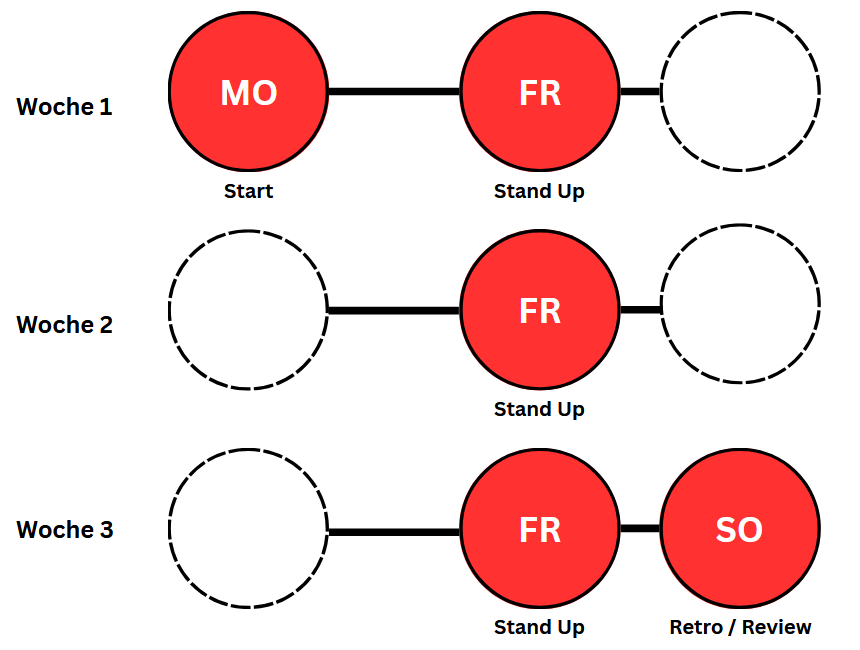
\includegraphics[width=0.85\linewidth]{Sprint_Zyklus.png}
  \caption{Ablauf eines 3-wöchigen Sprints}
  \label{fig:sprint-ablauf}
\end{figure}

\subsection{Kanban-Board}
Unser Board besteht aus \textbf{vier Spalten}, durch die alle Tickets von links nach rechts wandern:
\begin{itemize}[nosep]
  \item \textbf{Zu erledigen} — startklare Aufgaben
  \item \textbf{In Arbeit} — aktuell bearbeitete Aufgaben
  \item \textbf{Testing/Review} — Ergebnisse in Prüfung/Abnahme
  \item \textbf{Fertig} — abgeschlossene Aufgaben
\end{itemize}




\begin{figure}[H]
  \centering
  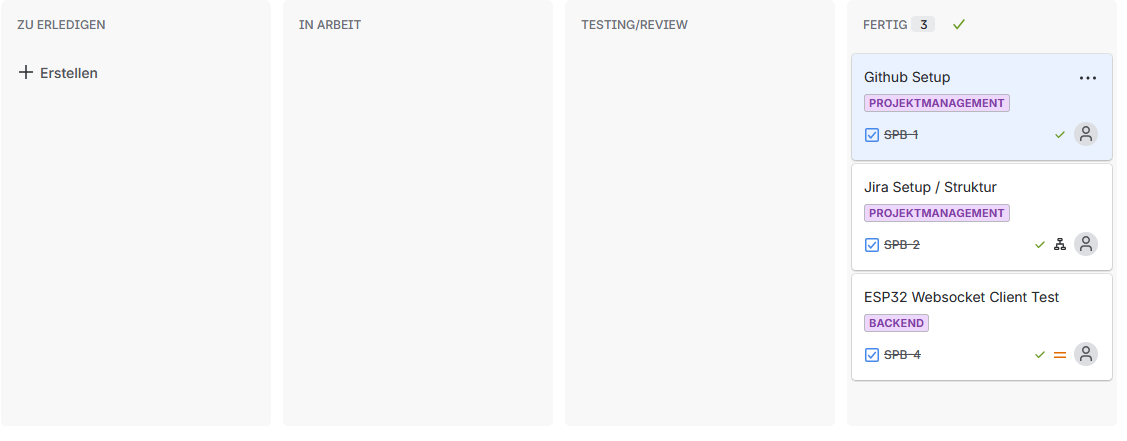
\includegraphics[width=\textwidth]{Kanban_Board_1_Sprint.png}
  \caption{Kanban-Board vom 22.09.2025}
  \label{fig:kanban-board-1-sprint}
\end{figure}

\begin{figure}[H]
  \centering
  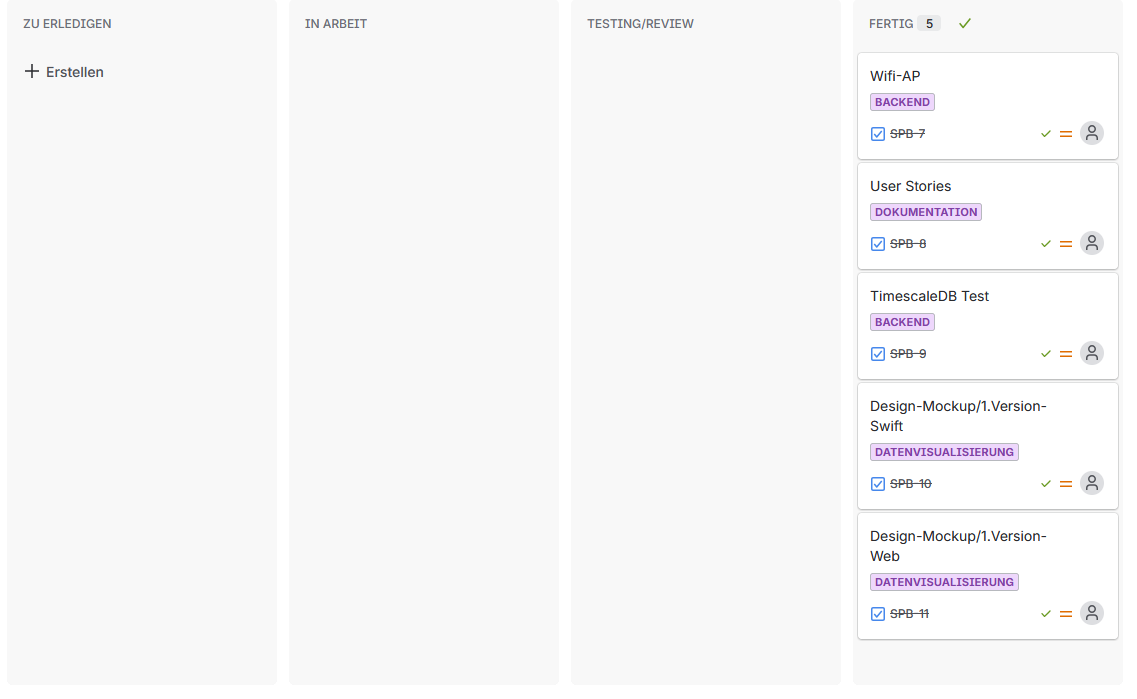
\includegraphics[width=\textwidth]{Kanban_Board_2_Sprint.png}
  \caption{Kanban-Board vom 13.10.2025}
  \label{fig:kanban-board-2-sprint}
\end{figure}

\begin{figure}[H]
  \centering
  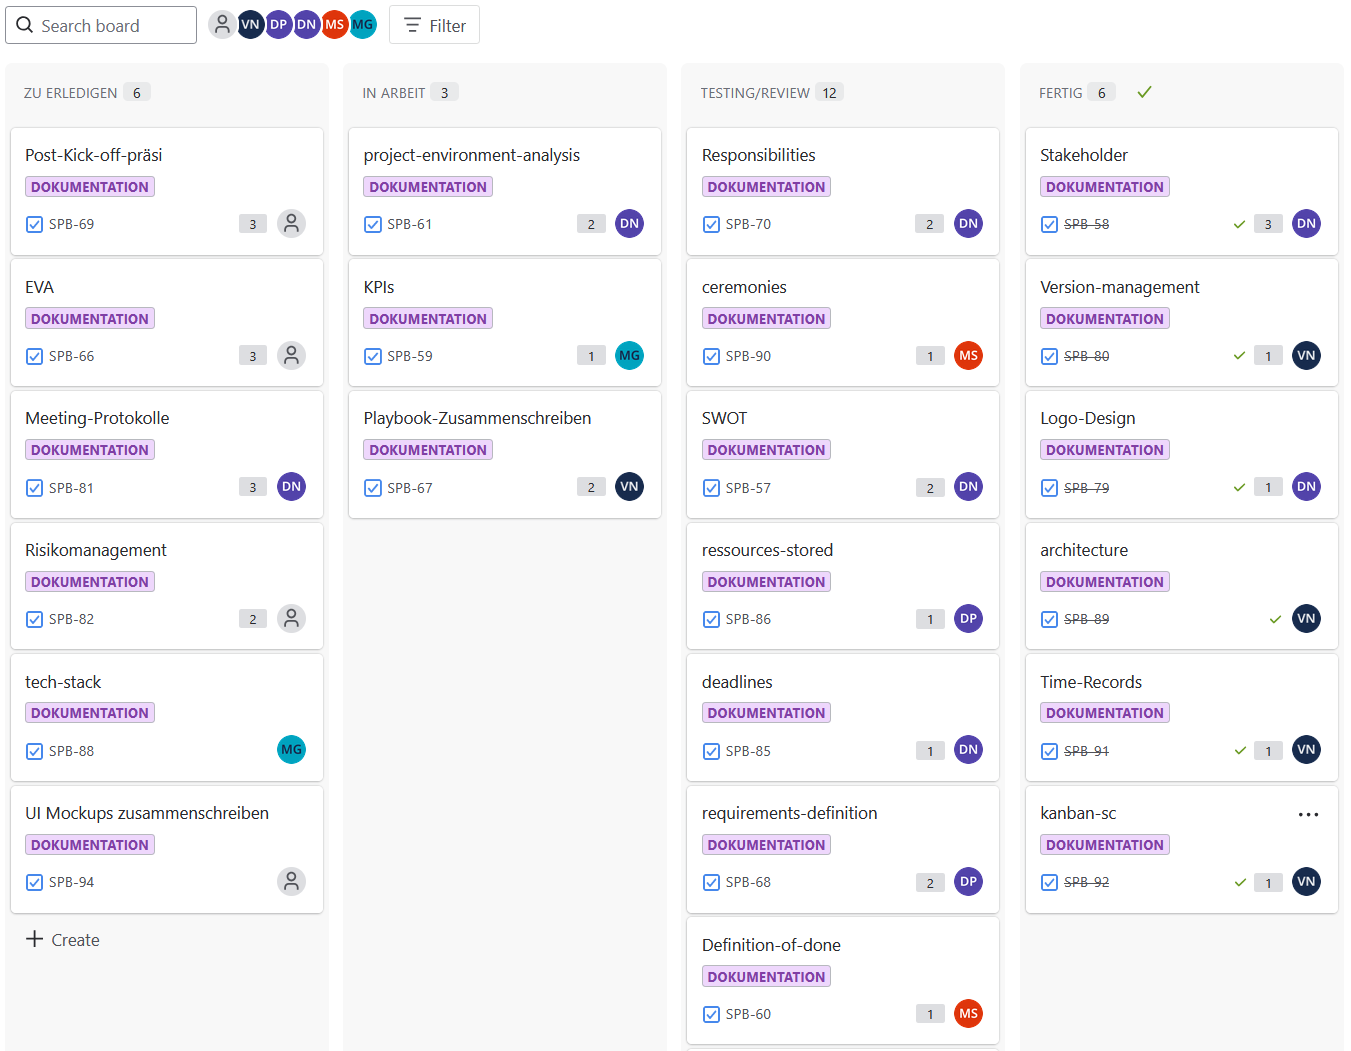
\includegraphics[width=\textwidth]{Kanban_Board_3_Sprint.png}
  \caption{Kanban-Board vom 20.10.2025}
  \label{fig:kanban-board-3-sprint}
\end{figure}


\pagebreak

\subsection{Project KPIs}

\subsubsection{Spillover-Rate}
\begin{description}
  \item[Definition:] Misst, wie viele Jira-Vorgänge in den nächsten Sprint übernommen werden.
  
  \item[Berechnung:] 
  \[
    \text{SpilloverRate} = 
    \frac{\text{Anzahl unvollständiger Vorgänge eines Sprints}}
         {\text{Anzahl gesamter Vorgänge eines Sprints}} 
    \times 100
  \]
  
  \item[Ziel:] Die Spillover-Rate hilft, die Selbsteinschätzung der Arbeitskapazität zu beurteilen.
\end{description}


\subsubsection{Deadline-Verfehlungen}
\begin{description}
  \item[Definition:] Anzahl der verfehlten Deadlines.
  \item[Ziel:] Die Anzahl der Deadline-Verfehlungen gibt Auskunft über die Effizienz des Projekts und die Selbsteinschätzungsfähigkeit des Projektteams.
\end{description}

\subsubsection{Teamzufriedenheit}
\begin{description}
  \item[Definition:] Durchschnittliche Zufriedenheit basierend auf einer Team-Umfrage.
  \item[Berechnung:] Durchschnitt der Bewertungen aller Mitglieder auf einer Skala von 1--10.
  \item[Ziel:] Die Teamzufriedenheit spiegelt das Projektumfeld wider. Bei niedrigen Werten können nach einer Teamdiskussion Maßnahmen abgeleitet werden, um Stimmung und Arbeitsbedingungen zu verbessern.
\end{description}



\subsection{Project Environment Analysis}

\begin{figure}[H]
  \centering
  \includesvg[width=\textwidth]{Project_Environment}
  \caption{Darstellung – Project Environment Analysis}
  \label{fig:project_environment_analysis}
\end{figure}

\pagebreak
\subsubsection*{Extern}
\begin{itemize}
  \item \textbf{Partneranforderungen.} BearingPoint definiert spezifische Anforderungen an das Projekt, z.\,B. den Einsatz bestimmter Sensoren oder technischer Standards. Diese Vorgaben dienen als Grundlage für die technische Umsetzung und werden regelmäßig überprüft, damit die Ergebnisse den Erwartungen des Partners entsprechen.
  \item \textbf{Technologische Abhängigkeiten.} Das Projekt ist auf bestimmte Technologien, Plattformen und Hardwarekomponenten angewiesen, die teilweise von externen Anbietern stammen. Änderungen oder Lieferverzögerungen dieser Abhängigkeiten können den Projektfortschritt beeinflussen und müssen frühzeitig erkannt und eingeplant werden.
  \item \textbf{Sonderanfertigung von Messgeräten.} Die Beschaffung und gegebenenfalls Sonderanfertigung von Sensoren sowie ESP32-Geräten kann längere Lieferzeiten mit sich bringen. Diese Aspekte sind frühzeitig in der Projektplanung zu berücksichtigen, um Verzögerungen in der Integrations- und Testphase zu vermeiden.
  \item \textbf{Rechtliche Vorgaben.} Bei der Entwicklung und Nutzung technischer Komponenten sind rechtliche Bestimmungen, insbesondere Urheberrecht und Datenschutz-Grundverordnung (DSGVO), einzuhalten. Dies betrifft sowohl die Nutzung von Softwarebibliotheken als auch den Umgang mit personenbezogenen Daten.
\end{itemize}

\subsubsection*{Projektbegleitend}
\begin{itemize}
  \item \textbf{Dokumentation \& Reporting.} Um Transparenz und Nachvollziehbarkeit zu gewährleisten, wird das Projekt umfassend dokumentiert. Dazu zählen regelmäßige Reports, Protokolle nach Meetings und Fortschrittsberichte, die den Projektverlauf festhalten und Entscheidungen begründen.
  \item \textbf{Feedback.} Regelmäßiges Feedback von BearingPoint und dem schulischen Projektbegleiter dient der Qualitätssicherung und ermöglicht frühzeitige Anpassungen im Entwicklungsprozess.
  \item \textbf{Transparenz im Entwicklungsprozess.} Der Fortschritt wird nachvollziehbar über \emph{Jira}, \emph{GitHub} und regelmäßige Reviews dargestellt.
  \item \textbf{Qualitätsmanagement.} Durch regelmäßige Tests, Code-Reviews und Validierungen wird sichergestellt, dass die Ergebnisse den definierten Anforderungen entsprechen und eine hohe technische sowie funktionale Qualität aufweisen.
\end{itemize}

\subsubsection*{Intern}
\begin{itemize}
  \item \textbf{Wissenstransfer.} Ein kontinuierlicher Austausch von Fachwissen, Ideen und Erfahrungen zwischen den Teammitgliedern unterstützt den Lernprozess und fördert die Effektivität der Zusammenarbeit. So können Auffälligkeiten schnell geklärt werden.
  \item \textbf{Codequalität.} Der Code wird nach klar definierten Best Practices entwickelt, getestet und dokumentiert. Dies sichert langfristige Wartbarkeit, Stabilität und Nachvollziehbarkeit für zukünftige Projektphasen oder Erweiterungen.
  \item \textbf{Motivation.} Hohe Eigenmotivation und Verantwortungsbewusstsein sind entscheidend für den Projekterfolg. Eigeninitiative, Engagement und Teamgeist helfen, Herausforderungen gemeinsam zu bewältigen.
  \item \textbf{Teamkommunikation.} Strukturierte und regelmäßige Kommunikation über digitale Plattformen wie \emph{Discord} oder \emph{Microsoft Teams} ermöglicht effiziente Abstimmung, schnelle Entscheidungen und fördert ein gemeinsames Verständnis im Team.
\end{itemize}






\subsection{Stakeholder Analysis}

\begin{figure}[H]
  \centering
  \includesvg[width=\textwidth]{Stakeholder_Analysis}
  \caption{Stakeholder Analysis — Übersicht}
  \label{fig:swot-produkt}
\end{figure}


\subsection{Stakeholder Mapping}

\begin{figure}[H]
\centering
\begin{tikzpicture}[scale=0.95]
  \colorlet{ringA}{red!10}
  \colorlet{ringB}{red!18}
  \colorlet{ringC}{red!30}
  \tikzset{
    labelStyle/.style={font=\bfseries\large, text=black!60},
    person/.style={font=\small, align=center, text=black}
  }

  \def\Rout{8.6}
  \def\Rmid{6.0}
  \def\Rin{3.8}

  \fill[ringA] (0,0) circle (\Rout);
  \fill[ringB] (0,0) circle (\Rmid);
  \fill[ringC] (0,0) circle (\Rin);

  \node[labelStyle] at (0,{(\Rout+\Rmid)/2}) {Informed};
  \node[labelStyle] at (0,{(\Rmid+\Rin)/2})  {Involved};
  \node[labelStyle] at (0,0)                 {Core Team};

  \node[person] at (-2.5,  0.7) {Daniel\\Nebel};
  \node[person] at ( 2.5,  0.7) {Matthias\\Gregorich};
  \node[person] at (-1.7, -1.7) {Damjan\\Petrovic};
  \node[person] at ( 1.7, -1.7) {Marc\\Schneeweis};
  \node[person] at ( 0.0, 2.5) {Viktor\\Novak};

  \node[person] at (-4.9, 1.1) {Helmut\\Vogl};
  \node[person] at ( 4.9, 1.1) {Thomas\\Prikryl};

  \node[person] at (-7.0,  2.0) {Harald\\Zumpf};
  \node[person] at ( 7.0,  2.0) {Nada\\Hasewend};
  \node[person] at ( 0.0, -7.3) {Dolezal\\Michael};
\end{tikzpicture}
\caption{Stakeholder Mapping — Übersicht}
\end{figure}

\begin{description}[leftmargin=2.8cm,style=nextline]
  \item[Core Team] Vollzeit im Team bzw.\ am Projekt arbeitend.
  \item[Involved] Hilft gelegentlich dabei, die Arbeit voranzubringen; dieses Projekt ist nicht ihr einziger Schwerpunkt.
  \item[Informed] Will auf dem Laufenden gehalten werden und hilft, wenn es nötig ist.
\end{description}






\subsection{Responsibilities}

Die Zuteilung der Verantwortlichkeiten im \textit{SensorBear}-Projekt orientiert sich an den verschiedenen Projektaspekten. So erhält jede Aufgabe die notwendige Aufmerksamkeit und jede Person kann in ihrem gewünschten Fachbereich arbeiten.

\begin{itemize}
  \item \textbf{Matthias Gregorich \textendash{} Infrastruktur und Datenschnittstellen:} Implementiert die Systeminfrastruktur sowie Schnittstellen zur Kommunikation zwischen Sensoren, Clients und Datenspeicherung. Bewertet und wählt geeignete Technologien für Persistierung und Datenübertragung. Zentral für den Aufbau einer skalierbaren, robusten und effizienten Backend-Struktur.
  
  \item \textbf{Daniel Nebel \textendash{} Mobile Applikation:} Verantwortlich für die Entwicklung der mobilen Anwendung des Projekts. Fokus auf benutzerfreundliches Design, hohe Performance und eine intuitive UI/UX für die Darstellung von Messdaten. Ziel ist eine einfache Navigation und ein optimales Nutzererlebnis auf mobilen Endgeräten.
  
  \item \textbf{Viktor Novak \textendash{} Qualitätssicherung und Automatisierung:} Entwickelt Strategien zur Qualitätssicherung und Automatisierung projektspezifischer Anwendungen. Schwerpunkt auf automatisierten Testverfahren zur Verbesserung der Codequalität. Zusätzlich Umsetzung einer Desktop-Applikation mit Electron, die Echtzeit-Push-Benachrichtigungen und erweiterte Datenansichten ermöglicht.
  
  \item \textbf{Damjan Petrovic \textendash{} Netzwerk- und Sensorkomponenten:} Verantwortlich für die Konstruktion und Programmierung von ESP32-basierten Sensorknoten in einem Mesh-Netzwerk. Der Fokus liegt auf zuverlässiger Kommunikation, stabiler Datenübertragung und Integration der Sensoren in das Gesamtsystem (Pairing). Fundamentaler Beitrag zur Schaffung der Hardware- und Kommunikationsbasis des Projekts.
  
  \item \textbf{Marc Schneeweis \textendash{} Web-Dashboard-Entwicklung:} Konzipiert und entwickelt ein webbasiertes Dashboard zur Visualisierung von Live-Daten, Statistiken und Warnmeldungen. Fokus auf klare Informationsdarstellung, intuitive Benutzeroberfläche und performante Datenanbindung. Trägt wesentlich zu einer transparenten und reaktionsschnellen Datenvisualisierung bei.
\end{itemize}





\subsection{Project Health Monitors}

\begin{figure}[H]
  \centering
  \includesvg[width=\textwidth]{Project_Health}
  \caption{Project Health Monitors}
  \label{fig:project_health_monitors}
\end{figure}


\subsection{SWOT Analysis}

\subsubsection{SWOT — Produkt}
\begin{figure}[H]
  \centering
  \includesvg[width=\textwidth]{SWOT_Produkt}
  \caption{SWOT-Analyse — Produkt}
  \label{fig:swot-produkt}
\end{figure}

\noindent\textbf{Strengths}
\begin{itemize}
  \item \textbf{Individualisiert:} Das Produkt ist auf die Bedürfnisse sowie auf das Bürogebäude von BearingPoint (Wiedner Gürtel~13/Turm~24, 1100~Wien) zugeschnitten.
  \item \textbf{Einfache modulare Sensorerweiterung:} Für Erweiterungen bestehender oder neuer Räume stehen neue „Plug-and-Play“-Sensoren bereit, die mittels „Pairing Mode“ schnell und unkompliziert konfiguriert werden können.
  \item \textbf{Individuell anpassbar:} Verbundene Benutzerinnen und Benutzer können Grenzwerte, Push-Benachrichtigungen und das Design nach ihren jeweiligen Anforderungen festlegen.
  \item \textbf{Intuitives Monitoring:} Optimierte, benutzerfreundliche Visualisierungen der Sensordaten ermöglichen eine übersichtliche und wirksame Überwachung.
\end{itemize}

\noindent\textbf{Weaknesses}
\begin{itemize}
  \item \textbf{Hardwareinstabilität:} Überhitzung an besonders heißen Tagen, Verschmutzung oder Abdeckung der Sensoren können den Datenfluss beeinträchtigen.
  \item \textbf{Zeitintensive Fertigung neuer Sensoren:} Erweiterungen über die fünf bereitgestellten Messgeräte hinaus erfordern Bestellung zusätzlicher Sensoren und ESP32, das Drucken passender Gehäuse sowie die Konfiguration des zusammengesetzten Messgeräts — ein zeitaufwändiger Prozess.
\end{itemize}

\pagebreak
\noindent\textbf{Opportunities}
\begin{itemize}
  \item \textbf{Bessere Luftqualität:} Die CO\textsubscript{2}-Messung und entsprechende Hinweise bei Unter- bzw.\ Überschreitung fördern eine bessere Raumluft.
  \item \textbf{Bessere Arbeitsatmosphäre:} Empfohlene Grenzwerte — angelehnt an \emph{WHO}-Empfehlungen und Metastudien — unterstützen eine optimale, produktive Arbeitsumgebung.
  \item \textbf{Ausbau des Produkts:} BearingPoint kann die bereitgestellten Daten und das System als Grundlage für zukünftige Erweiterungen und neue Funktionen nutzen.
\end{itemize}

\noindent\textbf{Threats}
\begin{itemize}
  \item \textbf{Geringe Sensorreichweite:} Bei großen Büroflächen mit niedriger Messgerätedichte kann das Mesh-Netz instabil werden.
  \item \textbf{Mesh-Interferenzen:} Externe Mesh-Netzwerke, verwinkelte Gebäude oder Stahlbetonwände können zu Störungen im Mesh-Netzwerk führen.
  \item \textbf{Nur Nahbereichszugriff:} Die Bedienung des Produkts ist auf den Nahbereich des aufgespannten Mesh-Netzwerks beschränkt.
\end{itemize}


\subsubsection{SWOT — Team}
\begin{figure}[H]
  \centering
  \includesvg[width=\textwidth]{SWOT_Team}
  \caption{SWOT-Analyse — Team}
  \label{fig:swot-team}
\end{figure}

\pagebreak
\noindent\textbf{Strengths}
\begin{itemize}
  \item \textbf{IoT-Erfahrung:} Alle Teammitglieder verfügen aus der HTL-Spengergasse über zwei Jahre Erfahrung in der IoT-Entwicklung.
  \item \textbf{Kollaboratives Team:} Benötigt ein Mitglied eine zweite Meinung oder Starthilfe, stehen andere, in diesem Bereich bewanderte, Teammitglieder bereit.
  \item \textbf{Schnelle Entscheidungsfindung:} Bei offenen Punkten wird ein Meeting einberufen, Vor- und Nachteile werden abgewogen und zeitnah die bestmögliche Entscheidung getroffen.
\end{itemize}

\noindent\textbf{Weaknesses}
\begin{itemize}
  \item \textbf{Begrenzte Praxiserfahrung:} Die Erfahrung an Produktivsystemen beläuft sich bei jedem Teammitglied auf etwa zwei Monate.
  \item \textbf{Begrenzte Zeitverfügbarkeit:} Durch die laufende Ausbildung an der HTL Spengergasse ist die verfügbare Arbeitszeit eingeschränkt.
  \item \textbf{Begrenztes Budget/Material:} Begrenzte finanzielle und materielle Ressourcen schränken Investitionen und Skalierung ein.
\end{itemize}

\noindent\textbf{Opportunities}
\begin{itemize}
  \item \textbf{Moderne Technologien:} Mit PostgreSQL, Swift, Next.js etc.\ arbeiten wir mit modernen Technologien, die eine bestmögliche Benutzererfahrung ermöglichen.
  \item \textbf{Experten-Ratgeber:} Mit Thomas Prikryl (BearingPoint-Entwickler) steht ein erfahrener und kompetenter Ratgeber im Development-Bereich zur Verfügung.
  \item \textbf{Wachsendes Unternehmensinteresse:} Ein erfolgreiches, zufriedenstellendes Produkt öffnet die Tür für zukünftige Zusammenarbeit.
\end{itemize}

\noindent\textbf{Threats}
\begin{itemize}
  \item \textbf{Abhängigkeit vom Partner:} Für die Installation des Mesh-Netzwerks sind wir auf das Bürogebäude von BearingPoint angewiesen; Büroumstellungen oder ein Umzug können zu Konflikten führen.
  \item \textbf{Interessenskonflikte mit dem Partner:} Meinungsverschiedenheiten zu Features oder deren Umsetzung können Risiken für den Projektfortschritt darstellen.
\end{itemize}







\subsection{Earned Value Analysis}

\begin{figure}[H]
  \centering
  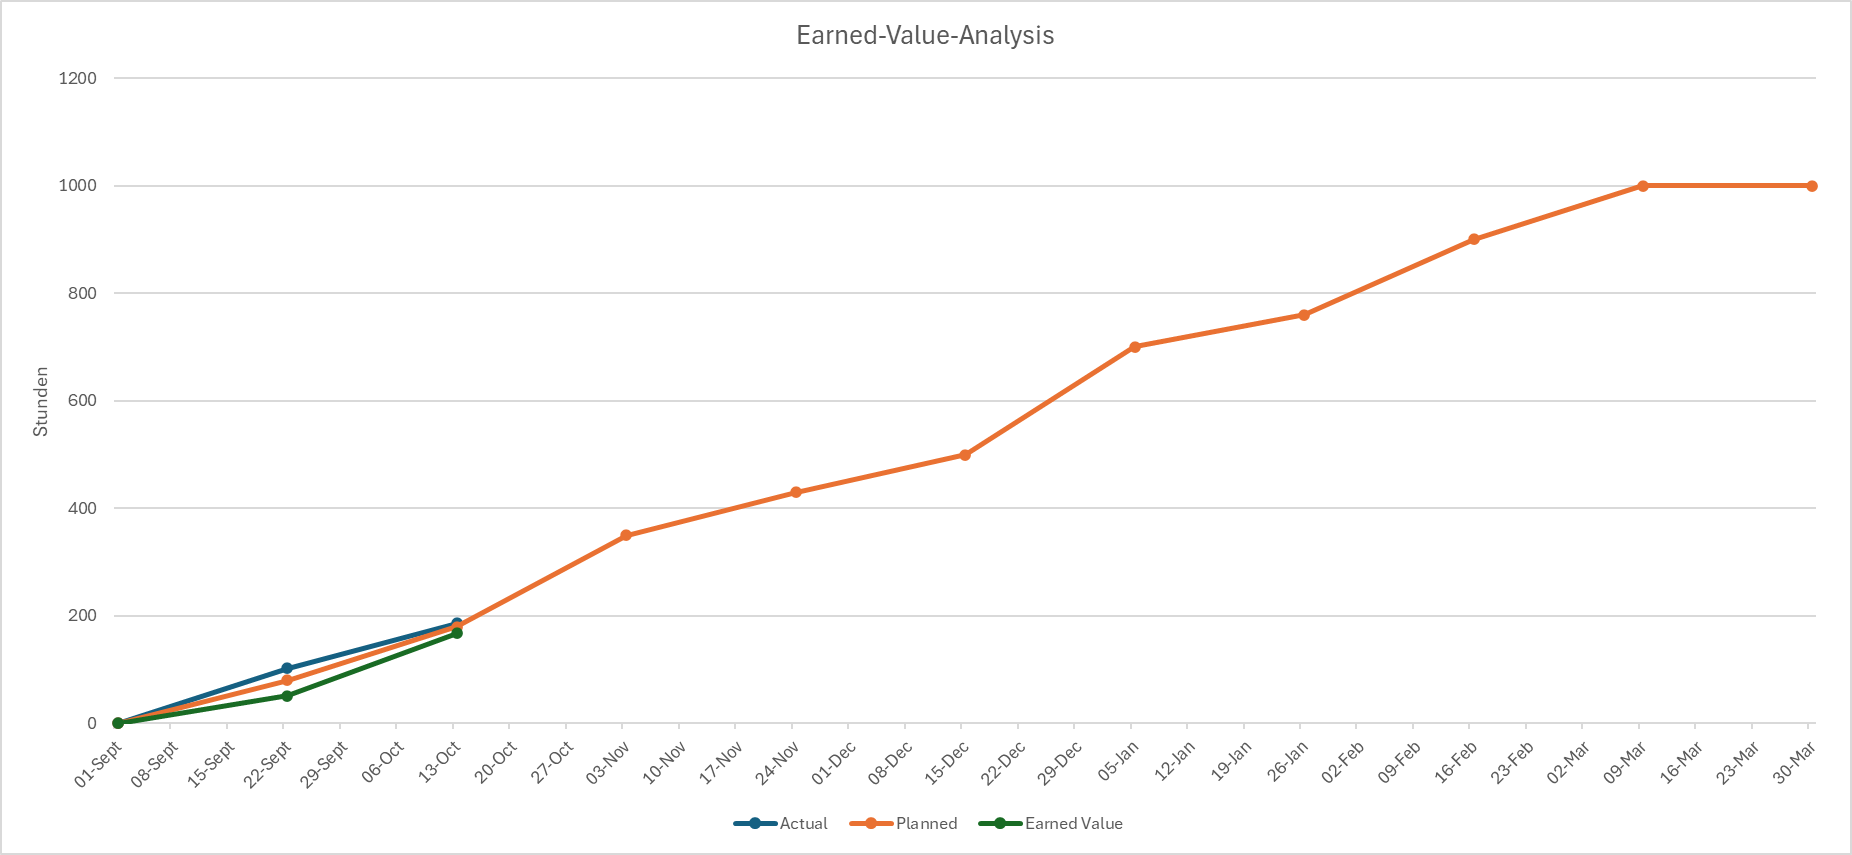
\includegraphics[width=\textwidth]{EVA.png}
  \caption{Darstellung – Earned Value Analysis}
  \label{fig:eva}
\end{figure}






\subsection{Ceremonies}
Wir haben als Team beschlossen, keine zusätzlichen Zeremonien abzuhalten, abseits der zuvor definierten Sprint-Parameter. Sollte jemand ein Meeting verpassen, informiert die betroffene Person das Team so früh wie möglich (z.B. über Discord oder Whatsapp). Verpasste Informationen werden anschließend im Stand Up oder über das Meeting Protokoll nachgeholt. Wenn eine Person krank ist und ihre zugeteilten Aufgaben nicht abschließen kann, werden diese an Teammitglieder verteilt, die das entsprechende Themengebiet gut beherrschen. Wenn Aufgaben keine Dringlichkeit haben dann werden diese auf den nächsten Sprint verschoben.





\subsection{Version Management Approach}

Der gesamte Code wird mit \textbf{Git} auf \textbf{GitHub} verwaltet.
Die einzelnen Komponenten sind in separaten \textbf{Repositories} organisiert.

\subsubsection{Branches}
\begin{itemize}
  \item \textbf{\branch{main}}: enthält jederzeit die stabile Release-Version. Auf diesem Branch werden keine direkten Commits ausgeführt, sondern nur Merges von \branch{dev}.
  \item \textbf{\branch{dev}}: enthält den aktuellen, noch ungetesteten bzw. instabilen Entwicklungsstand und dient als Basis für \branch{feature}.
  \item \textbf{\branch{feature}}: neue Features werden in diesen Branches pro Jira-Task (z.\,B. \texttt{feature/SPB-123-signin-form}) entwickelt und nach Abschluss der Entwicklung in \branch{dev} gemergt.
\end{itemize}











\section{Attachments}
\subsection{Compliance Guidelines}

Das Projekt ist vollständig \textbf{DSGVO-konform} und erfüllt alle Anforderungen an Datenschutz und Datensicherheit. 
Erfasst werden ausschließlich physikalische Umgebungsdaten (Temperatur, CO\textsubscript{2}-Konzentration, Luftfeuchtigkeit, Schalldruckpegel) ohne jeglichen Personenbezug. 
Die Kommunikation erfolgt ausschließlich innerhalb eines geschlossenen, internetfreien lokalen Netzwerks zwischen Sensorgeräten, Backend und Frontend. 
Technisch bedingte IP- und MAC-Adressen dienen nur der internen Gerätekommunikation, werden nicht gespeichert. 
Alle Messwerte werden lokal gespeichert, Benutzerkonten oder personenbezogene Logins existieren nicht. 
Damit wird höchste Datensouveränität gewährleistet und die Einhaltung der Datenschutz-Grundverordnung sichergestellt.






\subsection{Meeting Protocols}

\begin{table}[H]
  \centering
  \begin{tabularx}{\textwidth}{|>{\columncolor{black!10}}l|X|}
    \hline
    \textbf{Datum} & 01.09.2025 \\
    \hline
    \textbf{Teilnehmer intern} & Matthias Gregorich, Daniel Nebel, Viktor Novak, Damjan Petrovic, Marc Schneeweis \\ 
    \hline
    \textbf{Teilnehmer extern} & Nada Hasewend, Thomas Prikryl, Mladen Stefanovic  \\
    \hline
    \textbf{Ort} & Teams \\ 
    \hline
    \textbf{Ziel} &
    \vspace{-0.5em}
    \begin{itemize}
        \item Gegenseitiges Kennenlernen
        \item Thema/Idee Pitchen: IOT-Sensor Idee vorstellen und Meinungen einholen
    \end{itemize} \\
    \hline
    \textbf{Besprochene Punkte} &
    \vspace{-0.5em}
    \begin{itemize}
        \item Kommunikationswege festgelegt
        \item IOT-Sensor Projekt fixiert, mit dedizierter Web/Mobile Anzeige
    \end{itemize} \\
    \hline
    \textbf{Nächste Schritte} &
    \vspace{-0.5em}
    \begin{itemize}
        \item Gewünschte Features festlegen auf beiden Seiten
        \item PowerPoint für technische Umsetzung erstellen, für Meeting am 05.09.2025
    \end{itemize} \\
    \hline
  \end{tabularx}
  \caption{Meeting Protokoll vom 01.09.2025}
  \label{tab:meeting-01-09-2025}
\end{table}





\begin{table}[H]
  \centering
  \begin{tabularx}{\textwidth}{|>{\columncolor{black!10}}l|X|}
    \hline
    \textbf{Datum} & 02.09.2025 \\
    \hline
    \textbf{Teilnehmer intern} & Matthias Gregorich, Daniel Nebel, Viktor Novak, Damjan Petrovic, Marc Schneeweis \\ 
    \hline
    \textbf{Teilnehmer extern} & - \\
    \hline
    \textbf{Ort} & HTL Spengergasse \\ 
    \hline
    \textbf{Ziel} &
    \vspace{-0.5em}
    \begin{itemize}
        \item Ziel von Sprint 1 definieren
        \item Tickets/Features definieren 
        \item Aufgaben zuteilen
    \end{itemize} \\
    \hline
    \textbf{Besprochene Punkte} &
    \vspace{-0.5em}
    \begin{itemize}
        \item Setup/Struktur von Jira und Github
        \item Core-Features
        \item Vorstudie/Technologievergleich
        \item Hardwareumsetzung
    \end{itemize} \\
    \hline
    \textbf{Nächste Schritte} &
    \vspace{-0.5em}
    \begin{itemize}
        \item Features in User Stories festhalten
        \item Sprint 1 Start
    \end{itemize} \\
    \hline
  \end{tabularx}
  \caption{Meeting Protokoll vom 02.09.2025}
  \label{tab:meeting-02-09-2025}
\end{table}






\begin{table}[H]
  \centering
  \begin{tabularx}{\textwidth}{|>{\columncolor{black!10}}l|X|}
    \hline
    \textbf{Datum} & 05.09.2025 \\
    \hline
    \textbf{Teilnehmer intern} & Matthias Gregorich, Daniel Nebel, Viktor Novak, Damjan Petrovic, Marc Schneeweis \\ 
    \hline
    \textbf{Teilnehmer extern} & Nada Hasewend, Thomas Prikryl \\
    \hline
    \textbf{Ort} & Wiedner Gürtel 13/Turm 24, 1100 Wien/BearingPoint-Büro \\ 
    \hline
    \textbf{Ziel} &
    \vspace{-0.5em}
    \begin{itemize}
        \item Gewünschte Features austauschen und finalisieren
        \item Technologien fixieren
        \item Zeitplan absprechen
    \end{itemize} \\
    \hline
    \textbf{Besprochene Punkte} &
    \vspace{-0.5em}
    \begin{itemize}
        \item Features
          \begin{itemize}[label=-,leftmargin=1.2em,nosep,topsep=0pt]
            \item Raumplanung
            \item Sensor Mesh Integration
            \item Push Nachrichten
            \item Arten der Sensordatenanzeige
            \item Modulare Erweiterung für neue Sensoren/Räume
            \item Widgets
          \end{itemize}
        \item Freiraum/Einstellungsoptionen der Benutzer
        \item Technologische Umsetzung
        \item Kooperationsvertrag
    \end{itemize} \\
    \hline
    \textbf{Nächste Schritte} &
    \vspace{-0.5em}
    \begin{itemize}
        \item Vorstudien beginnen 
    \end{itemize} \\
    \hline
  \end{tabularx}
  \caption{Meeting Protokoll vom 05.09.2025}
  \label{tab:meeting-05-09-2025}
\end{table}







\begin{table}[H]
  \centering
  \begin{tabularx}{\textwidth}{|>{\columncolor{black!10}}l|X|}
    \hline
    \textbf{Datum} & 25.09.2025 \\
    \hline
    \textbf{Teilnehmer intern} & Matthias Gregorich, Daniel Nebel, Viktor Novak \\ 
    \hline
    \textbf{Teilnehmer extern} & - \\
    \hline
    \textbf{Ort} & HTL Spengergasse \\ 
    \hline
    \textbf{Ziel} &
    \vspace{-0.5em}
    \begin{itemize}
        \item Kommunikation unter den Schnittstellen und ESPs klären
        \item Zeitintervall festlegen
    \end{itemize} \\
    \hline
    \textbf{Besprochene Punkte} &
    \vspace{-0.5em}
    \begin{itemize}
        \item Websocketumsetzung
          \begin{itemize}[label=-,leftmargin=1.2em,nosep,topsep=0pt]
            \item Echtzeitdatenverkehr
            \item Zeitintervalle per Endpoint
          \end{itemize}
        \item Ausfall von ESPs 
        \item Datenwiderherstellung
        \item Raumplandarstellung in Backend und Frontend
        \item Hinzufügen neuer ESPs in bestehendes oder neues Mesh ("Pairing-Mode")
    \end{itemize} \\
    \hline
    \textbf{Nächste Schritte} &
    \vspace{-0.5em}
    \begin{itemize}
        \item UI Mockups
        \item Database Struktur
    \end{itemize} \\
    \hline
  \end{tabularx}
  \caption{Meeting Protokoll vom 25.09.2025}
  \label{tab:meeting-25-09-2025}
\end{table}






\begin{table}[H]
  \centering
  \begin{tabularx}{\textwidth}{|>{\columncolor{black!10}}l|X|}
    \hline
    \textbf{Datum} & 17.10.2025 \\
    \hline
    \textbf{Teilnehmer intern} & Matthias Gregorich, Daniel Nebel, Viktor Novak, Marc Schneeweis \\ 
    \hline
    \textbf{Teilnehmer extern} & - \\
    \hline
    \textbf{Ort} & Discord \\ 
    \hline
    \textbf{Ziel} &
    \vspace{-0.5em}
    \begin{itemize}
        \item Dokumentation aufteilen
        \item Dokumentation Umsetzung
    \end{itemize} \\
    \hline
    \textbf{Besprochene Punkte} &
    \vspace{-0.5em}
    \begin{itemize}
        \item Project Management Report Aufgaben
        \item Design des Reports
        \item Zuteilung
        \item Deadlines der einzelnen Aufgaben
    \end{itemize} \\
    \hline
    \textbf{Nächste Schritte} &
    \vspace{-0.5em}
    \begin{itemize}
        \item Dokumentation bearbeiten
    \end{itemize} \\
    \hline
  \end{tabularx}
  \caption{Meeting Protokoll vom 17.10.2025}
  \label{tab:meeting-17-10-2025}
\end{table}


\subsection{Time Records}


\begin{figure}[H]
  \centering
  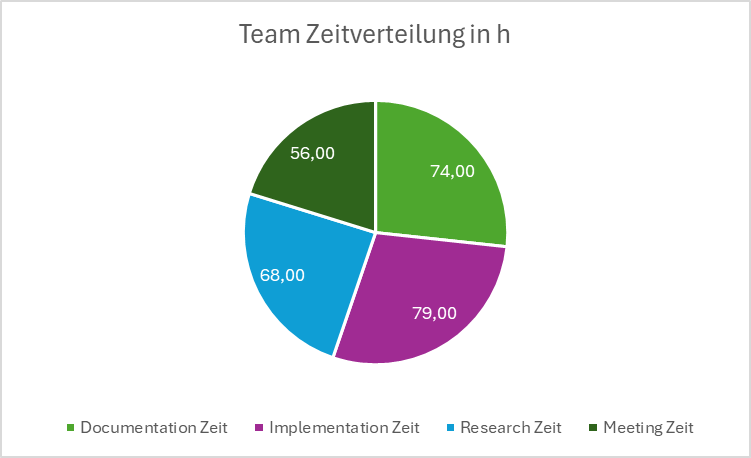
\includegraphics[width=\textwidth]{Team_Zeitdarstellung.png}
  \caption{Team-Zeitdarstellung}
  \label{fig:team-zeitdarstellung}
\end{figure}



\subsubsection*{Matthias Gregorich}

\begin{figure}[H]
  \centering
  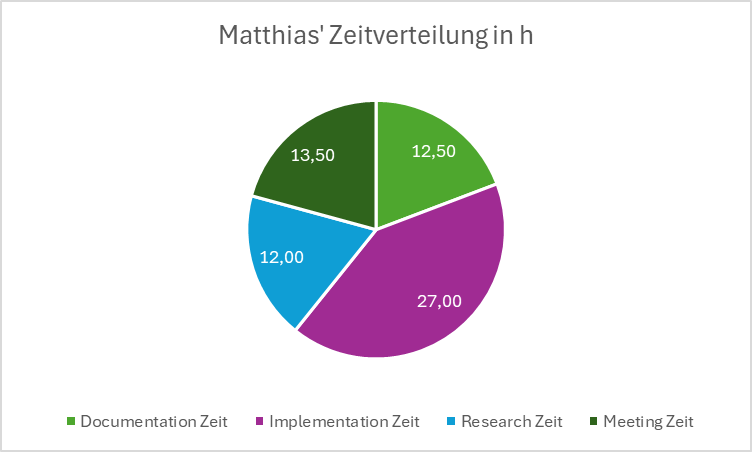
\includegraphics[width=\textwidth]{Matthias_Zeitverteilung.png}
  \caption{Zeitverteilung – Matthias Gregorich}
  \label{fig:matthias-zeitverteilung}
\end{figure}

\begin{table}[H]
  \centering
  \begin{tabularx}{\textwidth}{|c|c|c|X|}
    \hline
    \rowcolor{black!10}\textbf{Datum} & \textbf{Dauer} & \textbf{Kategorie} & \textbf{Beschreibung} \\
    \hline
    01.09.2025 & 2:00:00 & Meeting           & BearingPoint Absprache 1 \\ \hline
    02.09.2025 & 2:00:00 & Meeting           & Unterricht Vorbereitungsphase/Sprint 1 Meeting \\ \hline
    03.09.2025 & 1:00:00 & Research          & Unterricht Vorbereitungsphase \\ \hline
    03.09.2025 & 1:00:00 & Projektmanagement & Github aufsetzen \\ \hline
    04.09.2025 & 2:00:00 & Research          & Unterricht Vorbereitungsphase \\ \hline
    05.09.2025 & 3:00:00 & Meeting           & BearingPoint Absprache 2 \\ \hline
    10.09.2025 & 1:00:00 & Research          & Unterricht Vorbereitungsphase \\ \hline
    11.09.2025 & 2:00:00 & Research          & Unterricht Vorbereitungsphase \\ \hline
    16.09.2025 & 2:00:00 & Research          & Unterricht Vorbereitungsphase \\ \hline
    17.09.2025 & 1:00:00 & Research          & Unterricht Vorbereitungsphase \\ \hline
    19.09.2025 & 4:00:00 & Implementierung   & C\# WebSocket Implementation \\ \hline
    19.09.2025 & 1:00:00 & Research          & Unterricht Vorbereitungsphase \\ \hline
    20.09.2025 & 5:00:00 & Implementierung   & ESP32 WebSocket Client Test mit C\# Backend \\ \hline
    22.09.2025 & 3:00:00 & Projektmanagement & Jira-Setup und erste User-Stories erstellt \\ \hline
    23.09.2025 & 2:00:00 & Implementierung   & ESP32 WIFI-AP Firmware \\ \hline
    23.09.2025 & 2:00:00 & Research          & Unterricht Vorbereitungsphase \\ \hline
    24.09.2025 & 3:00:00 & Implementierung   & ESP32 WIFI-AP DHCP + Testing \\ \hline
    25.09.2025 & 2:00:00 & Meeting           & Umsetzung von Techstack \\ \hline
    26.09.2025 & 2:30:00 & Projektmanagement & Jira Board Besprechung \\ \hline
    02.10.2025 & 2:00:00 & Implementierung   & TimescaleDB Setup + Testing \\ \hline
    03.10.2025 & 1:00:00 & Implementierung   & Unterricht Vorstudie, Development \\ \hline
    04.10.2025 & 2:00:00 & Implementierung   & First Entity definition + First Endpoints Created \\ \hline
    07.10.2025 & 3:00:00 & Implementierung   & Unterricht Vorstudie, Development \\ \hline
    10.10.2025 & 1:00:00 & Implementierung   & Unterricht Vorstudie, Development \\ \hline
    14.10.2025 & 2:00:00 & Implementierung   & Unterricht Vorstudie, Development \\ \hline
    15.10.2025 & 1:00:00 & Implementierung   & Unterricht Vorstudie, Development \\ \hline
    15.10.2025 & 2:30:00 & Projektmanagement & Jira Tasks (Techstack, Architecture) \\ \hline
    16.10.2025 & 2:30:00 & Projektmanagement & Jira Tasks (KPIs, Version Mangement) \\ \hline
    17.10.2025 & 1:00:00 & Implementierung   & Unterricht Vorstudie, Development \\ \hline
    17.10.2025 & 2:00:00 & Meeting           & Playbook Besprechung \\ \hline
    20.10.2025 & 3:30:00 & Projektmanagement & Jira Tasks (Techstack, Architecture) überarbeitet \\ \hline
    \rowcolor{black!10}\textbf{Summe} & \textbf{65:00:00} & & \\ \hline
  \end{tabularx}
  \caption{Zeitaufzeichnung – Matthias Gregorich}
  \label{tab:zeit-matthias}
\end{table}



\subsubsection*{Daniel Nebel}

\begin{figure}[H]
  \centering
  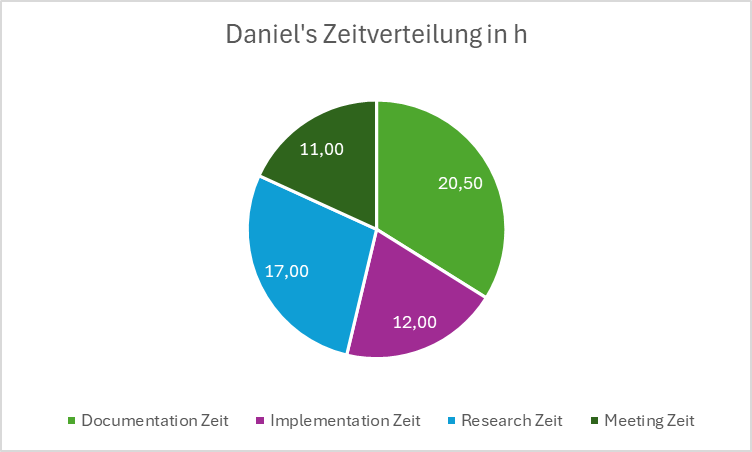
\includegraphics[width=\textwidth]{Daniel_Zeitverteilung.png}
  \caption{Zeitverteilung – Daniel Nebel}
  \label{fig:daniel-zeitverteilung}
\end{figure}


\begin{table}[H]
  \centering
  \begin{tabularx}{\textwidth}{|c|c|c|X|}
    \hline
    \rowcolor{black!10}\textbf{Datum} & \textbf{Dauer} & \textbf{Kategorie} & \textbf{Beschreibung} \\
    \hline
    01.09.2025 & 2:00:00 & Meeting           & BearingPoint Absprache 1 \\ \hline
    02.09.2025 & 2:00:00 & Meeting           & Unterricht Vorbereitungsphase/Sprint 1 Meeting \\ \hline
    03.09.2025 & 1:00:00 & Research          & Unterricht Vorbereitungsphase \\ \hline
    03.09.2025 & 1:00:00 & Projektmanagement & Github aufsetzen \\ \hline
    04.09.2025 & 2:00:00 & Research          & Unterricht Vorbereitungsphase \\ \hline
    05.09.2025 & 3:00:00 & Meeting           & BearingPoint Absprache 2 \\ \hline
    10.09.2025 & 1:00:00 & Research          & Unterricht Vorbereitungsphase \\ \hline
    10.09.2025 & 3:00:00 & Research          & Swift-LiDAR/ARKit \\ \hline
    11.09.2025 & 2:00:00 & Research          & Unterricht Vorbereitungsphase \\ \hline
    16.09.2025 & 2:00:00 & Research          & Unterricht Vorbereitungsphase \\ \hline
    17.09.2025 & 1:00:00 & Research          & Unterricht Vorbereitungsphase \\ \hline
    19.09.2025 & 1:00:00 & Research          & Unterricht Vorbereitungsphase \\ \hline
    22.09.2025 & 3:00:00 & Projektmanagement & Jira-Setup und erste User-Stories erstellt \\ \hline
    23.09.2025 & 2:00:00 & Research          & Unterricht Vorbereitungsphase \\ \hline
    25.09.2025 & 2:00:00 & Meeting           & Umsetzung von Techstack \\ \hline
    26.09.2025 & 2:30:00 & Projektmanagement & Jira Board Besprechung \\ \hline
    30.09.2025 & 2:30:00 & Research          & Playbook (SWOT, Canva Visio, Stakeholder, PE) \\ \hline
    03.10.2025 & 1:00:00 & Implementierung   & Unterricht Vorstudie, Development \\ \hline
    05.10.2025 & 3:00:00 & Implementierung   & Figma Mockup \\ \hline
    07.10.2025 & 3:00:00 & Implementierung   & Unterricht Vorstudie, Development \\ \hline
    10.10.2025 & 1:00:00 & Implementierung   & Unterricht Vorstudie, Development \\ \hline
    14.10.2025 & 2:00:00 & Implementierung   & Unterricht Vorstudie, Development \\ \hline
    15.10.2025 & 1:00:00 & Implementierung   & Unterricht Vorstudie, Development \\ \hline
    17.10.2025 & 1:00:00 & Implementierung   & Unterricht Vorstudie, Development \\ \hline
    17.10.2025 & 2:00:00 & Meeting           & Playbook Besprechung \\ \hline
    18.10.2025 & 3:00:00 & Projektmanagement & Jira Tasks (Responsibilities, SWOT, Project Environment Analysis) \\ \hline
    19.10.2025 & 3:00:00 & Projektmanagement & Jira Tasks (Stakeholder, Deadlines) \\ \hline
    20.10.2025 & 5:00:00 & Projektmanagement & Meetingprotokolle aufbereiten, Projekt-Logo, Playbook schreiben \\ \hline
    20.10.2025 & 3:00:00 & Projektmanagement & Post Kickoff Präsentation \\ \hline
    \rowcolor{black!10}\textbf{Summe} & \textbf{60:30:00} & & \\ \hline
  \end{tabularx}
  \caption{Zeitaufzeichnung – Daniel Nebel}
  \label{tab:zeit-daniel}
\end{table}


\subsubsection*{Viktor Novak}

\begin{figure}[H]
  \centering
  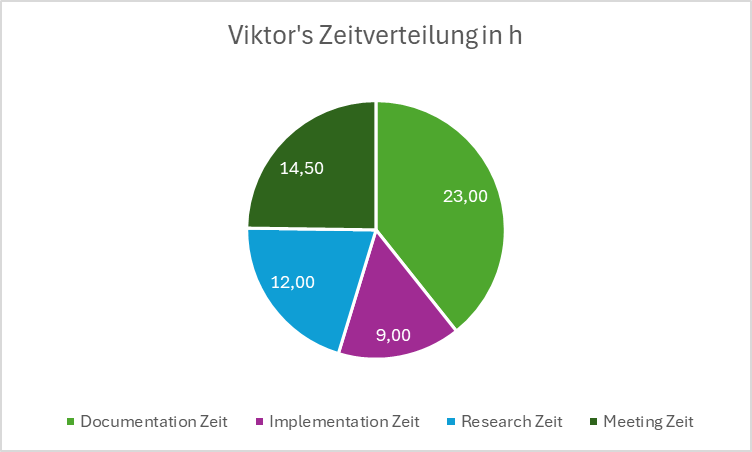
\includegraphics[width=\textwidth]{Viktor_Zeitverteilung.png}
  \caption{Zeitverteilung – Viktor Novak}
  \label{fig:viktor-zeitverteilung}
\end{figure}

\begin{table}[H]
  \centering
  \begin{tabularx}{\textwidth}{|c|c|c|X|}
    \hline
    \rowcolor{black!10}\textbf{Datum} & \textbf{Dauer} & \textbf{Kategorie} & \textbf{Beschreibung} \\
    \hline
    01.09.2025 & 2:00:00 & Meeting           & BearingPoint Absprache 1 \\ \hline
    02.09.2025 & 2:00:00 & Meeting           & Unterricht Vorbereitungsphase/Sprint 1 Meeting \\ \hline
    03.09.2025 & 1:00:00 & Research          & Unterricht Vorbereitungsphase \\ \hline
    03.09.2025 & 1:00:00 & Projektmanagement & Github aufsetzen \\ \hline
    04.09.2025 & 2:00:00 & Research          & Unterricht Vorbereitungsphase \\ \hline
    05.09.2025 & 3:00:00 & Meeting           & BearingPoint Absprache 2 \\ \hline
    10.09.2025 & 1:00:00 & Research          & Unterricht Vorbereitungsphase \\ \hline
    11.09.2025 & 2:00:00 & Research          & Unterricht Vorbereitungsphase \\ \hline
    16.09.2025 & 2:00:00 & Research          & Unterricht Vorbereitungsphase \\ \hline
    17.09.2025 & 1:00:00 & Research          & Unterricht Vorbereitungsphase \\ \hline
    19.09.2025 & 1:00:00 & Research          & Unterricht Vorbereitungsphase \\ \hline
    23.09.2025 & 2:00:00 & Research          & Unterricht Vorbereitungsphase \\ \hline
    25.09.2025 & 2:00:00 & Meeting           & Umsetzung von Techstack \\ \hline
    26.09.2025 & 2:30:00 & Projektmanagement & Jira Board Besprechung \\ \hline
    27.09.2025 & 1:00:00 & Research          & Umsetzung von Techstack \\ \hline
    03.10.2025 & 1:00:00 & Implementierung   & Unterricht Vorstudie, Development \\ \hline
    07.10.2025 & 3:00:00 & Implementierung   & Unterricht Vorstudie, Development \\ \hline
    10.10.2025 & 1:00:00 & Implementierung   & Unterricht Vorstudie, Development \\ \hline
    14.10.2025 & 2:00:00 & Implementierung   & Unterricht Vorstudie, Development \\ \hline
    15.10.2025 & 1:00:00 & Implementierung   & Unterricht Vorstudie, Development \\ \hline
    15.10.2025 & 2:30:00 & Projektmanagement & Jira Tasks (Techstack, Architecture) \\ \hline
    16.10.2025 & 2:30:00 & Projektmanagement & Jira Tasks (KPIs, Version Mangement) \\ \hline
    17.10.2025 & 1:00:00 & Implementierung   & Unterricht Vorstudie, Development \\ \hline
    17.10.2025 & 2:00:00 & Meeting           & Playbook Besprechung \\ \hline
    18.10.2025 & 8:00:00 & Projektmanagement & Playbook schreiben \\ \hline
    20.10.2025 & 6:00:00 & Projektmanagement & Playbook schreiben \\ \hline
    21.10.2025 & 2:30:00 & Projektmanagement & Playbook schreiben \\ \hline
    \rowcolor{black!10}\textbf{Summe} & \textbf{61:00:00} & & \\ \hline
  \end{tabularx}
  \caption{Zeitaufzeichnung – Viktor Novak}
  \label{tab:zeit-viktor}
\end{table}


\subsubsection*{Damjan Petrovic}

\begin{figure}[H]
  \centering
  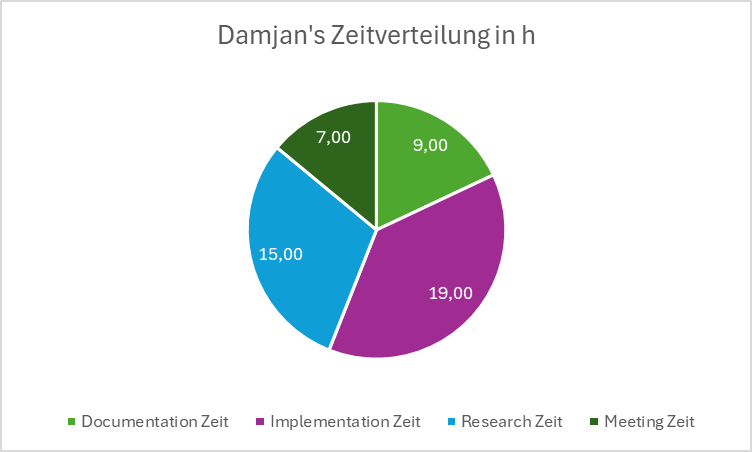
\includegraphics[width=\textwidth]{Damjan_Zeitverteilung.png}
  \caption{Zeitverteilung – Damjan Petrovic}
  \label{fig:damjan-zeitverteilung}
\end{figure}

\begin{table}[H]
  \centering
  \begin{tabularx}{\textwidth}{|c|c|c|X|}
    \hline
    \rowcolor{black!10}\textbf{Datum} & \textbf{Dauer} & \textbf{Kategorie} & \textbf{Beschreibung} \\
    \hline
    01.09.2025 & 2:00:00 & Meeting           & BearingPoint Absprache 1 \\ \hline
    02.09.2025 & 2:00:00 & Meeting           & Unterricht Vorbereitungsphase/Sprint 1 Meeting \\ \hline
    03.09.2025 & 1:00:00 & Research          & Unterricht Vorbereitungsphase \\ \hline
    03.09.2025 & 1:00:00 & Projektmanagement & Github aufsetzen \\ \hline
    04.09.2025 & 2:00:00 & Research          & Unterricht Vorbereitungsphase \\ \hline
    05.09.2025 & 3:00:00 & Meeting           & BearingPoint Absprache 2 \\ \hline
    10.09.2025 & 1:00:00 & Research          & Unterricht Vorbereitungsphase \\ \hline
    11.09.2025 & 2:00:00 & Research          & Unterricht Vorbereitungsphase \\ \hline
    16.09.2025 & 2:00:00 & Research          & Unterricht Vorbereitungsphase \\ \hline
    17.09.2025 & 1:00:00 & Research          & Unterricht Vorbereitungsphase \\ \hline
    19.09.2025 & 1:00:00 & Research          & Unterricht Vorbereitungsphase \\ \hline
    22.09.2025 & 3:00:00 & Research          & Vorstudie Sensoren \\ \hline
    23.09.2025 & 2:00:00 & Research          & Unterricht Vorbereitungsphase \\ \hline
    23.09.2025 & 3:00:00 & Implementierung   & Planung Sensorgehäuse \\ \hline
    27.09.2025 & 2:00:00 & Implementierung   & Planung Sensorgehäuse \\ \hline
    03.10.2025 & 1:00:00 & Implementierung   & Unterricht Vorstudie, Development \\ \hline
    03.10.2025 & 3:00:00 & Implementierung   & ESP32 Sensor Chip Test \\ \hline
    07.10.2025 & 3:00:00 & Implementierung   & Unterricht Vorstudie, Development \\ \hline
    10.10.2025 & 1:00:00 & Implementierung   & Unterricht Vorstudie, Development \\ \hline
    14.10.2025 & 2:00:00 & Implementierung   & Unterricht Vorstudie, Development \\ \hline
    15.10.2025 & 1:00:00 & Implementierung   & Unterricht Vorstudie, Development \\ \hline
    17.10.2025 & 1:00:00 & Implementierung   & Unterricht Vorstudie, Development \\ \hline
    17.10.2025 & 2:00:00 & Implementierung   & ESP32 Sensor Chip Test \\ \hline
    19.10.2025 & 3:00:00 & Projektmanagement & Jira Tasks (Ressources Stored, Requirements Definition, Collaboration Approach) \\ \hline
    20.10.2025 & 2:00:00 & Projektmanagement & Jira Tasks (Ressources Stored, Requirements Definition, Collaboration Approach) \\ \hline
    20.10.2025 & 3:00:00 & Projektmanagement & Post Kickoff Präsentation \\ \hline
    \rowcolor{black!10}\textbf{Summe} & \textbf{50:00:00} & & \\ \hline
  \end{tabularx}
  \caption{Zeitaufzeichnung – Damjan Petrovic}
  \label{tab:zeit-damjan}
\end{table}


\subsubsection*{Marc Schneeweis}

\begin{figure}[H]
  \centering
  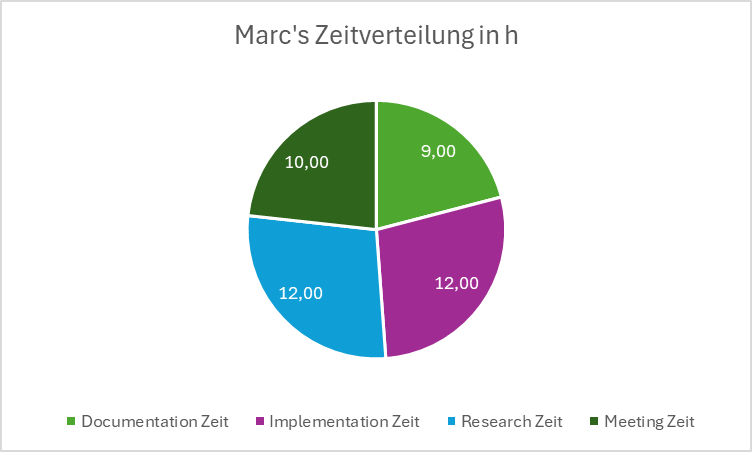
\includegraphics[width=\textwidth]{Marc_Zeitverteilung.png}
  \caption{Zeitverteilung – Marc Schneeweis}
  \label{fig:marc-zeitverteilung}
\end{figure}

\begin{table}[H]
  \centering
  \begin{tabularx}{\textwidth}{|c|c|c|X|}
    \hline
    \rowcolor{black!10}\textbf{Datum} & \textbf{Dauer} & \textbf{Kategorie} & \textbf{Beschreibung} \\
    \hline
    01.09.2025 & 2:00:00 & Meeting           & BearingPoint Absprache 1 \\ \hline
    02.09.2025 & 2:00:00 & Meeting           & Unterricht Vorbereitungsphase/Sprint 1 Meeting \\ \hline
    03.09.2025 & 1:00:00 & Research          & Unterricht Vorbereitungsphase \\ \hline
    03.09.2025 & 1:00:00 & Projektmanagement & Github aufsetzen \\ \hline
    04.09.2025 & 2:00:00 & Research          & Unterricht Vorbereitungsphase \\ \hline
    05.09.2025 & 3:00:00 & Meeting           & BearingPoint Absprache 2 \\ \hline
    10.09.2025 & 1:00:00 & Research          & Unterricht Vorbereitungsphase \\ \hline
    11.09.2025 & 2:00:00 & Research          & Unterricht Vorbereitungsphase \\ \hline
    16.09.2025 & 2:00:00 & Research          & Unterricht Vorbereitungsphase \\ \hline
    17.09.2025 & 1:00:00 & Research          & Unterricht Vorbereitungsphase \\ \hline
    19.09.2025 & 1:00:00 & Research          & Unterricht Vorbereitungsphase \\ \hline
    23.09.2025 & 2:00:00 & Research          & Unterricht Vorbereitungsphase \\ \hline
    27.09.2025 & 1:00:00 & Research          & Umsetzung von Techstack \\ \hline
    03.10.2025 & 1:00:00 & Implementierung   & Unterricht Vorstudie, Development \\ \hline
    05.10.2025 & 3:00:00 & Implementierung   & Figma Mockup \\ \hline
    07.10.2025 & 3:00:00 & Implementierung   & Unterricht Vorstudie, Development \\ \hline
    10.10.2025 & 1:00:00 & Implementierung   & Unterricht Vorstudie, Development \\ \hline
    14.10.2025 & 2:00:00 & Implementierung   & Unterricht Vorstudie, Development \\ \hline
    15.10.2025 & 1:00:00 & Implementierung   & Unterricht Vorstudie, Development \\ \hline
    17.10.2025 & 1:00:00 & Implementierung   & Unterricht Vorstudie, Development \\ \hline
    17.10.2025 & 2:00:00 & Meeting           & Playbook Besprechung \\ \hline
    19.10.2025 & 2:00:00 & Projektmanagement & Jira Tasks (Project Health, Ceremonies und Definition of Done) \\ \hline
    20.10.2025 & 3:00:00 & Projektmanagement & Jira Tasks (Sprintparameter) \\ \hline
    20.10.2025 & 3:00:00 & Projektmanagement & Post Kickoff Präsentation \\ \hline
    21.10.2025 & 1:30:00 & Projektmanagement & Playbook schreiben \\ \hline
    \rowcolor{black!10}\textbf{Summe} & \textbf{44:30:00} & & \\ \hline
  \end{tabularx}
  \caption{Zeitaufzeichnung – Marc Schneeweis}
  \label{tab:zeit-marc}
\end{table}



\subsectiontitlepage{Cooperation Contract}
\includepdfnopagenum[pages=-,fitpaper=true]{Kooperationsvereinbarung_BearingPoint.pdf}

\subsectiontitlepage{Legal Declaration}
\includepdfnopagenum[pages=-,fitpaper=true]{Rechtliche_Erklaerung.pdf}

\subsectiontitlepage{Software Requirements Specification}
\includepdfnopagenum[pages=-,fitpaper=true]{Requirements.pdf}


\end{document}
